\documentclass{nthuthesis}

\usepackage{times}
\usepackage{verbatim}
\usepackage{color}
\usepackage{url}
\usepackage{graphicx}
\usepackage{array}
\usepackage{wallpaper} 
\usepackage{cite}
\usepackage{caption}

\usepackage{multirow}
\usepackage{makecell}
\usepackage{hhline}
\usepackage{rotating}
\usepackage{amsmath}
\usepackage{amssymb}
\usepackage{mathrsfs}

% declare the path(s) where your graphic files are
\graphicspath{{./figsrc/}}
% and their extensions so you won't have to specify these with
% every instance of \includegraphics
\DeclareGraphicsExtensions{.pdf,.jpeg,.png}

% Using the tex-text mapping for ligatures etc.
\defaultfontfeatures{Mapping=tex-text}

% Set the default fonts

% English font
% Note: please refer to 'fc-list :outline -f "%{family}\n"' for choosing a valid font name
\setmainfont{Times New Roman}

% Chinese font
% Note: please refer to 'fc-list :outline -f "%{family}\n"' for choosing a valid font name
\setCJKmainfont[AutoFakeBold=3,AutoFakeSlant=.4]{Kaiti TC}
\defaultCJKfontfeatures{AutoFakeBold=6,AutoFakeSlant=.4}

\ifdefined\withwatermark
  \CenterWallPaper{0.5}{watermark.pdf}
\fi

% Your information goes here
% author: Tz-Huan Huang [http://www.csie.ntu.edu.tw/~tzhuan]

% ----------------------------------------------------------------------------
% "THE CHOCOLATE-WARE LICENSE":
% Tz-Huan Huang wrote this file. As long as you retain this notice you
% can do whatever you want with this stuff. If we meet some day, and you think
% this stuff is worth it, you can buy me a chocolate in return Tz-Huan Huang
% ----------------------------------------------------------------------------

% Syntax: \var{English}{Chinese}
\university{National Tsing Hua University}{國立清華大學}
\college{College of Electrical Engineering and Computer Science}{電機資訊學院}
\institute{Institute of Information Systems and Applications}{資訊系統與應用研究所}
\division{系統}
\title{ An Algorithm improve on AOI System }{自動光學檢測系統的演算法改良}
\author{Hao-Jui Lu}{呂昊叡}
\studentid{105065527}
\advisor{Wing-Kai Hon}{韓永楷}
\defenseyear{2018}{107}
\defensemonth{July}{7}
\defenseday{10}


\begin{document}

\frontmatter

\makecover
\makecopyright


\begin{acknowledgementszh}
感謝\ldots
\end{acknowledgementszh}

\begin{acknowledgementsen}
I'm glad to thank\ldots 
\end{acknowledgementsen}

\begin{abstractzh}
在工業檢測的場合中,自動化影像辨識(AOI)技術日漸成為一個重要的應用,
而現成的影像處理軟體通常有授權費過高,且準確度與分析速度並不符合產線的預算與需求,
這份論文中,我們用開源的工具實作了一個低成本的解決方案,滿足產線對於分析速度的需求。
本研究所實作出的產品檢驗流程可以粗略分為兩步驟,
第一步驟為樣板設定,此步驟會紀錄標準的產品特徵;
第二步驟為樣本檢驗,此步驟會將樣本與第一步驟所記錄下的樣本進行比對,並判斷此背光鍵盤是否有瑕疵或故障。
本論文主要討論自動化光學檢測系統及分析演算法的設計架構與分析過程中的演算法比較並加以改良。
並在最後將嘗試過的各種方法以產線實際運作的標準下進行比較。

\end{abstractzh}

\begin{abstracten}
In the industrial production site, Automatic-Optics-Inspection (AOI) techniques has become an importent application.
Since the existing image processing software is not cost effective due to expensive licence fee, 
and doesn't meet the requirment of on speed and accuracy. 
In this thesis, we proposed a low cost solution implemented with open source tools.


\end{abstracten}


{\singlespacing
\tableofcontents
\listoffigures
\listoftables
}

\mainmatter
% Your thesis goes here
\chapter{Introduction}
\label{c:intro}

\section{Motivation}
<<<<<<< HEAD
Since the cost of existing software solution is too high, and has little flexibility while tunning algorithms.
The

\subsection{Previous Solution}
add previous work here.



\section{Related Works}
\label{section:related-work}
add referenced paper here and write some comment

\section{Goal}
\label{section:goal}
Design a system that is both cost efficient and time efficient. Could identify lettering defect and LED light defect on keyboard.
=======
\label{section:motivation}
High-tech tools are prevalent nowadays and many of our daily are now routinely performed with computers. People write articles with computers; people draw diagrams with computers; people, of course, design programs with computers. Among our various usages of computers, one of them is music composition. For the purpose of storing and visualizing musicians' creation, the standard western musical score, which contains information pertaining to how a piece of music should be played, has been used for hundreds of years and around the globe. However, the score was designed for human beings instead of computers, and most of scores are scanned and stored as images, which means nothing but lots of pixels for computers. In other words, these scores are not yet symbolically represented. Therefore, the concern of this dissertation is \emph{optical music recognition} (OMR), which refers to the development of methods that automatically convert score images into their symbolic representation.

\section{Goal}
\label{section:goal}
Design a software that converts a score image (.png / .jpeg / .bmp / .pdf) into its symbolic representation encoded in a format that is readable by a computer such as MusicXML.
>>>>>>> parent of 2a4e8fe... updated

\section{Divide and Conquer}
% \subsection{Definition}
% \label{section:divide-and-conquer}

% Fig.~\ref{fig:DnC} shows the concepts of \emph{divide and conquer} (D\&C). D\&C is an algorithm design paradigm that breaks a complex problem into a couple of relatively simple subproblems, to \emph{divide}, then solves them respectively, to \emph{conquer}. Before conquering, the problem will be divided recursively until it is simple enough to be processed. Finally, the solutions to the subproblems will be merged as those to the original problem.

% \begin{figure}[!htb]
%     \centering
%     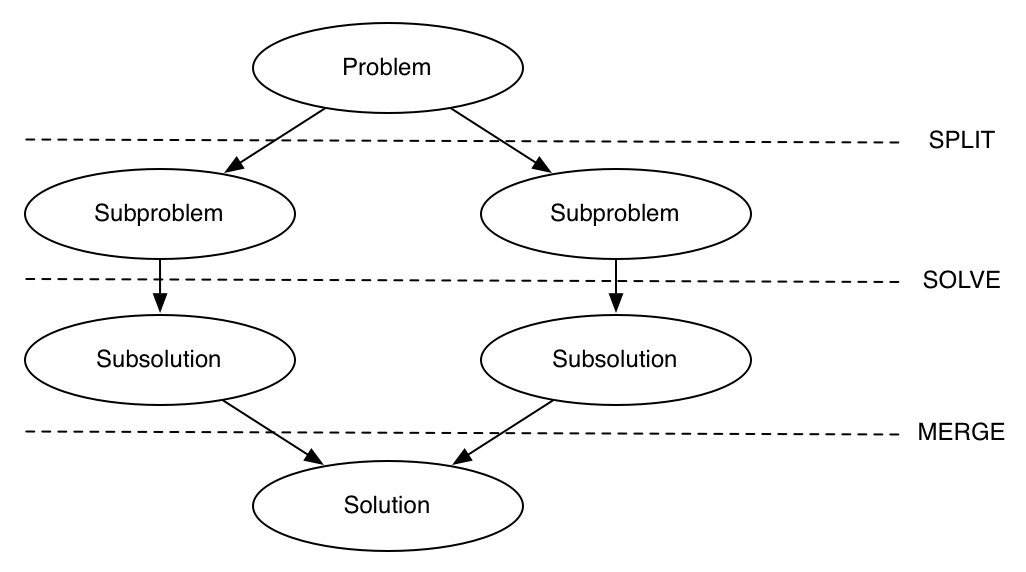
\includegraphics[width=\textwidth]{figsrc/DnC.png}
%     \caption{A diagram showing how divide and conquer works.\label{fig:DnC}}
% \end{figure}

\subsection{Main Contribution of This Dissertation}
\label{subsec:advantages}

\subsubsection{Reducing the Difficulty of Problems}

\subsubsection{Independence of Subproblems}

\subsubsection{Parallelism}


% Nowadays, a processor usually has multiple cores, and lots of computational tasks are implemented to be executed with parallel programs. In D\&C algorithm, the functions solving split subproblems are identically designed. With high independence and similar operations between subproblems, it is a good strategy to process them simultaneously. In other word, the original problem is suitable to be solved with \emph{SIMD (Single-Instruction-Multiple-Data)} parallel programs.

\chapter{Overview of System}
\label{c:overveiw-of-system}

In this section, previous works of OMR are mentioned. Preprocessing (binarization, staff profiling, staff detection, and staff removal) and recognition (symbol segmentation, symbol classification) are included. 

\section{Binarization}
% Binarization

% \begin{figure}[ht]
%     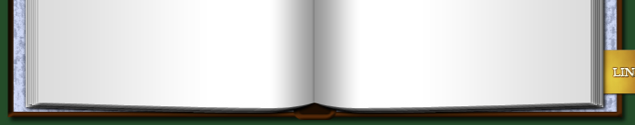
\includegraphics[width=\textwidth]{bookspine}
%     \caption{Example of the gray-scale image near the book spine\label{fig:bookspine}.}
% \end{figure}

\section{Staff Detection and Removal}

% Dalitz et al.~\cite{Dalitz:2008:CSoSRA} introduced a systematic way for testing the staff removal algorithms. A dataset was generated from a set of ideal score images with the deformation methods listed in Table.~\ref{table:deformation}. The deformation algorithms and the CVC-MUSCIMA dataset are made openly available by Forns et al.~\cite{Forns:2012:CVC-MUSCIMA}.

% \begin{table}[ht]
%     \hspace{-.5in}
%     \begin{tabular}{|c|c|c|}
%         \hline
%         {\bf Deformation} & {\bf Type} & {\bf Parameter Description} \\
%         \hline
%         Curvature & deterministic & height/width ratio of sine curve \\
%         \hline
%         Typeset Emulation & both & \parbox[c]{9cm}{gap width, maximal height and variance of vertical shift} \\
%         \hline
%         Line Interruptions & random & \parbox[c]{9cm}{interruption frequency, maximal width and variance of gap width} \\
%         \hline
%         Thickness Variation & random & \parbox[c]{9cm}{Markov chain stationary distribution and inertia factor} \\
%         \hline
%         $y$-variation & random & \parbox[c]{9cm}{Markov chain stationary distribution and inertia factor} \\
%         \hline
%         Degradation & random & \parbox[c]{9cm}{emulating local distortions suggested by Kanungo et al.~\cite{Kanungo:2000:Degradation}} \\
%         \hline
%         White Speckles & random & \parbox[c]{9cm}{speckle frequency, random walk length and smoothing factor} \\
%         \hline
%     \end{tabular}
%     \caption{Deformation Methods\label{table:deformation}.}
% \end{table}

\chapter{Discussion}
\label{c:disscussion}
% \chapter{Conclusion}
\label{c:intro}

\appendix

\backmatter

\renewcommand{\bibname}{References}
\addcontentsline{toc}{chapter}{\bibname}
\bibliographystyle{ieeetr}

% Your bibliography goes here
{\singlespacing
\bibliography{thesis}
}

\end{document}
